\documentclass[a4paper]{article}

\usepackage[english]{babel}
\usepackage[utf8x]{inputenc}
\usepackage{amsmath}
\usepackage{graphicx}
\usepackage[colorinlistoftodos]{todonotes}
\title{Joint Modeling of Content-Partitioned Multinetwork Embeddings (CPME) and Point Process Approach}
\author{Bomin Kim}

\begin{document}
\maketitle

\begin{abstract}
Your abstract.
\end{abstract}

\section{Ideas}
Current CPME model does not involve any of temporal component, which plays a key role in email interactions. Starting from the previous framework focused on the analysis of content-partitioned subnetworks, I would suggest an extended approach to analyze the data using the timestamps in the email, aiming to develop a joint dynamic or longitudinal model of text-valued ties.\\ \newline
 CPME model is a Bayesian framework using two methods: LDA and LSM. Basically, edges are based on topic t (LDA) and interaction pattern c (LSM). 
Each topic t=1,…,T has one interaction pattern c=1,…,C (e.g. broadcasting, meeting scheduling) and each interaction pattern has unique latent space. 
\newpage
\section{Preliminary Analysis}
\subsection{Dare County}
\footnotesize
\begin{table}[ht]
	\centering
	\begin{tabular}{ |c|ccc|c| } 
		\hline 
		\textbf{Period} &\textbf{Before Sandy} & \textbf{During Sandy} & \textbf{After Sandy} & \textbf{Overall} \\ 	\hline
			\textbf{\# emails}& 1933 & 1563 & 1467 & 4963 \\ 
		\hline
	\end{tabular}
	\caption{ Summary of Dare county email data based on time period}
	\label{table:nullDare2}
\end{table}
\normalsize
Before Sandy ranges from 2012-09-01 to 2012-10-21 (7 weeks), During Sandy ranges from 2012-10-22 to 2012-11-02 (2 weeks), and After Sandy ranges from 2012-11-03 to 2012-11-30 (4 weeks).
\footnotesize
\begin{figure}[ht]
	\centering
	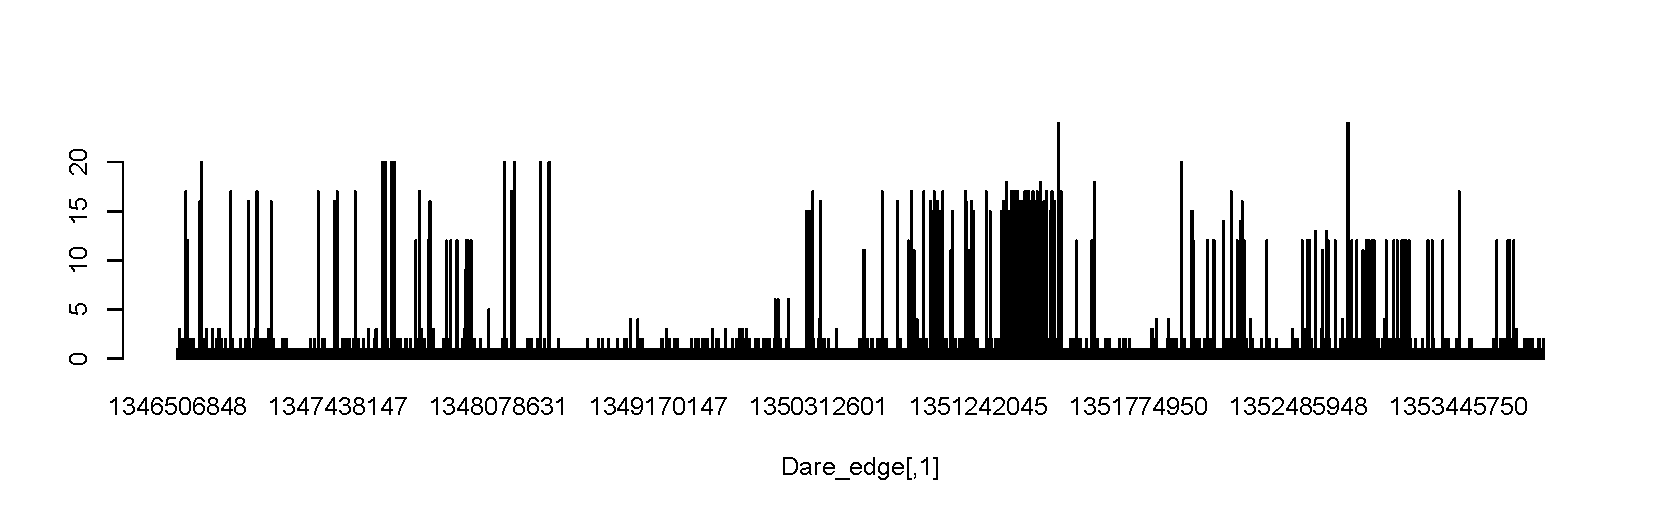
\includegraphics[width=1.1\textwidth]{DareEmails.pdf} 
	\caption{Frequency of Dare county emails from 2012-09-01 to 2012-11-30  }
	\label{fig:Emailplots}
\end{figure}
\begin{table}[ht]
	\centering
	\begin{tabular}{ |c|cc| } 
		\hline 
		\textbf{Time Interval} &\textbf{send} & \textbf{receive} \\ 	
		\hline  $[-\infty, t)$&  2.128, 2.659, 2.355, 2.919& 0.292, 0.257, 0.047, 0.110\\  $[t-30 m, t)$ &  0.262, -0.064, 0.782, 0.317 &2.087, 1.287 , 2.346, 1.870\\  $[t-2h, t-30m)$& 0.383, 0.157 , 0.024, -0.045 &0.553, 0.082, 0.794, 0.269\\ $[t-8h, t-2h)$ & 0.816, 0.054 , 0.077, 0.381 &-0.221, 0.048, 0.298, -0.012 \\ $[t-32h, t-8h)$& 0.085, 0.014,  0.228, 0.070 &0.101, 0.017, -0.033, 0.019\\ $[t-5.33d, t-32h)$&  0.103, 0.025, 0.092, 0.008 &-0.027, -0.016, -0.033, -0.009 \\ $[t-21.33d, t-5.33d)$  & 0.052, 0.000, 0.059, 0.010& 0.013, 0.030 , -0.016, 0.013\\ 
		$[-\infty, t-21.33d)$  & 0.052, 0.103, 0.027, 0.021  & 0.008, 0.000, 0.020, -0.005\\
		\hline
	\end{tabular}
	\caption {Estimated coefficients and approximate standard errors for dyadic effects of Dare county data (before Sandy, during Sandy, after Sandy, overall)}
	\label{table:nullDare}
\end{table}
\footnotesize
\begin{figure}[ht]
	\centering
	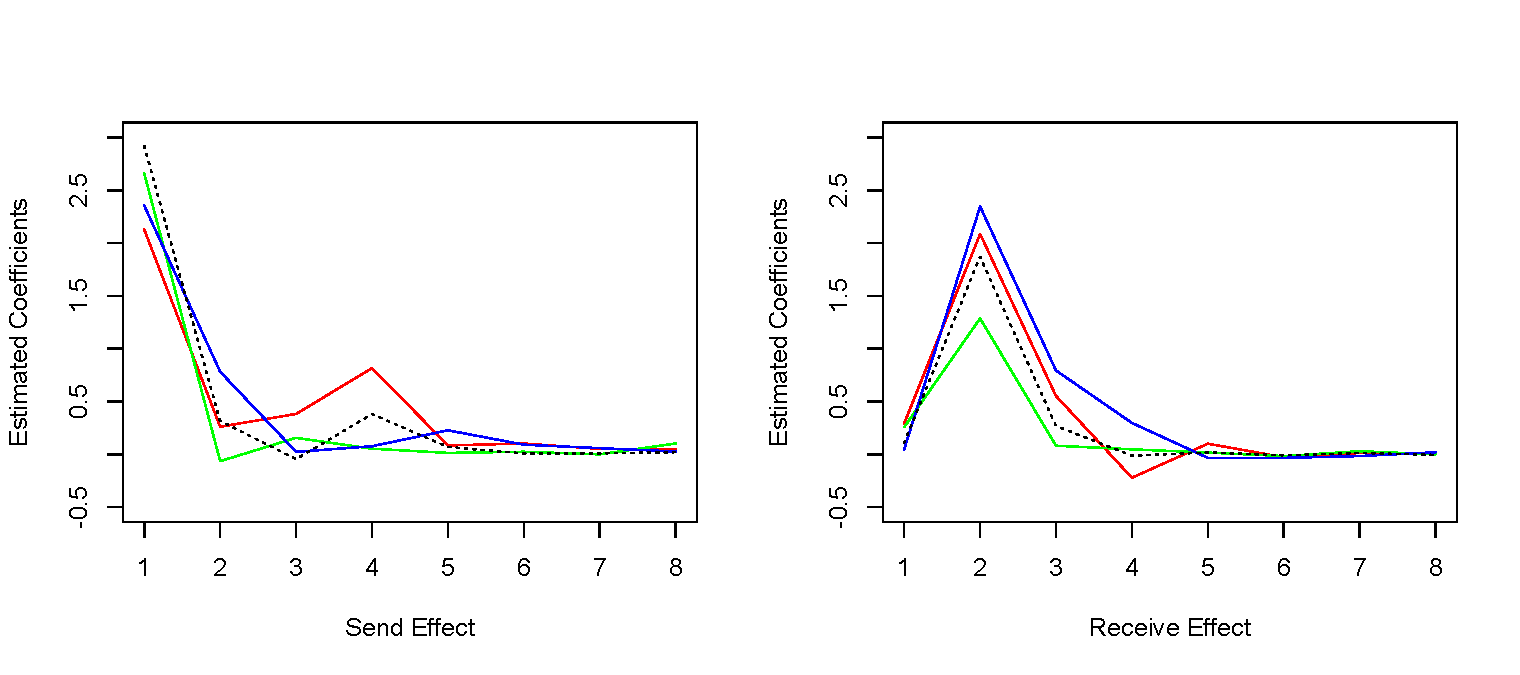
\includegraphics[width=1.1\textwidth]{Dareplot.pdf} 
	\caption{Comparison of Send (left) and Receive (right) effect based on periods in Table 1.}
	\label{fig:Emailplot}
\end{figure}
\newpage
\subsection{Lenoir County}
\footnotesize
\begin{table}[ht]
	\centering
	\begin{tabular}{ |c|cc| } 
		\hline 
		\textbf{Time Interval} &\textbf{send} & \textbf{receive} \\ 	
		\hline  $[-\infty, t)$&  2.543 (0.123)& 0.375 (0.084) \\  $[t-30 m, t)$ &  0.068 (0.117) &  1.956 (0.173) \\  $[t-2h, t-30m)$& 0.550 (0.158) & 0.839 (0.169)\\ $[t-8h, t-2h)$ & 0.781 (0.077)&  0.024 (0.075)\\ $[t-32h, t-8h)$& 0.208 (0.042)  &  0.112 (0.043)\\ $[t-5.33d, t-32h)$&  0.099 (0.027)& 0.091 (0.025)\\ $[t-21.33d, t-5.33d)$  & 0.043 (0.009) & -0.006 (0.008)\\ 
		$[-\infty, t-21.33d)$  & 0.051 (0.004)& -0.029 (0.004)  \\
		\hline
	\end{tabular}
	\caption {Estimated coefficients and approximate standard errors for dyadic effects of Lenoir county data}
	\label{table:nullLenoir}
\end{table}
\normalsize
\subsection{Vance County}
\footnotesize
\begin{table}[ht]
	\centering
	\begin{tabular}{ |c|cc| } 
		\hline 
		\textbf{Time Interval} &\textbf{send} & \textbf{receive} \\ 	
		\hline  $[-\infty, t)$&  2.543 (0.123)& 0.375 (0.084) \\  $[t-30 m, t)$ &  0.068 (0.117) &  1.956 (0.173) \\  $[t-2h, t-30m)$& 0.550 (0.158) & 0.839 (0.169)\\ $[t-8h, t-2h)$ & 0.781 (0.077)&  0.024 (0.075)\\ $[t-32h, t-8h)$& 0.208 (0.042)  &  0.112 (0.043)\\ $[t-5.33d, t-32h)$&  0.099 (0.027)& 0.091 (0.025)\\ $[t-21.33d, t-5.33d)$  & 0.043 (0.009) & -0.006 (0.008)\\ 
		$[-\infty, t-21.33d)$  & 0.051 (0.004)& -0.029 (0.004)  \\
		\hline
	\end{tabular}
	\caption {Estimated coefficients and approximate standard errors for dyadic effects of Vance county data}
	\label{table:nullVance}
\end{table}
\normalsize
\end{document}